\documentclass[11pt,a4paper]{article}
\usepackage[margin=2.0cm]{geometry}
\usepackage{graphicx,amsmath,amssymb,booktabs,xcolor,hyperref,float,caption,longtable,array}
\newcommand{\kT}{k_BT}\newcommand{\half}{\tfrac12}\newcommand{\la}{\ell_a}
\newcolumntype{P}[1]{>{\raggedright\arraybackslash}p{#1}}
\setlength{\parskip}{4pt}\setlength{\parindent}{0pt}
\title{Frank constants and flow coupling:\\ what changes in our claims}
\author{Survey for B.~Loewe, 21 October 2026 (before the static response test)}
\date{}
\begin{document}\maketitle

\section*{Summary}
\begin{itemize}
\item \textbf{New measurement.} With the director--flow coupling switched off (shear susceptibility $\chi_\mathrm{HI}=0$), the 2D MPCD nematic is isotropic:
$K_1=K_3=43.8\,\kT$, $K_1/K_3=1.00$, as Shendruk \& Yeomans found in 3D with the same switch. With the coupling on, the fluctuation constants follow the
flow-alignment parameter $\lambda$: $K_1/K_3=0.49$, 1.05, 1.49, 1.97 at $\lambda=-2$, 0, 1, 2. The flow softens the mode it rotates most; a mode with zero
coupling keeps the bare value. The rotational viscosity is unchanged, $\gamma_1\approx60$.
\item \textbf{The open question.} Do the defects respond to the bare isotropic stiffness, or to the effective anisotropic one? Two limiting readings
are used throughout:
\textbf{A} (bare): the anisotropy lives only in the noise (an anisotropic effective temperature); mean structures feel $K_1=K_3\approx44$.
\textbf{B} (effective): the flow coupling also renormalises the response; mean structures feel $K_1\approx43$, $K_3\approx22$.
The static response test (running) decides; the mode decay rates already hint at a partial response anisotropy (splay decays 1.2--1.5 times faster
than bend with the coupling on, 1.0--1.2 with it off, inverted at $\lambda=-2$), but they are noisy and confounded by backflow.
\item \textbf{One correction applies in both readings.} MPCD multiplies the Jeffery rotation by $\chi_\mathrm{HI}=0.5$, so the alignment length is
$\ell_E=\sqrt{K/(\chi_\mathrm{HI}\gamma_1 s\sqrt{\lambda^2-1})}$. Our MPCD $\ell_E$ omitted $\chi_\mathrm{HI}$ (too short by $\sqrt2$). The ``$+16^\circ$''
boundary-layer estimate did include it.
\item \textbf{What is at stake.} Under A, every statement that rests on splay $\neq$ bend loses its mechanism: site pinning (80--110\,$\kT$), the static tilt
potential and its sign change with crowding, ``elasticity alone gives $35^\circ$'', the $+2$--$3^\circ$ residual, and the static elastic pull invoked
for the crowding drop. Energies computed with one constant ($K=32.5$) scale by 1.35 with unchanged ratios and signs. Under B the existing numbers
stand (anisotropy-dependent ones grow by about 12\%), but the anisotropy must be described as a property of the flow-coupled algorithm, not as bare
elasticity.
\item \textbf{A tension that exists already.} Passive seeded rings ($2k-2$ plus bulk pair; runs/rest\_pinning, coupling on) kept tilts of 60 and
$120^\circ$ for 100--300\,t.u.\ with no pull back to $0^\circ$. That is hard to square with an 80--110\,$\kT$ barrier at zero tilt even in reading B,
and the relaxed anisotropic energies of the seeding generator already disagreed with the first-order barrier (they fall with the offset).
\item \textbf{What survives in both readings:} the lock $\tau_j=(2k-2)\phi_j+c$ and the $2|k-1|$ count; the leading tilt law $\arccos(1/\lambda)$; every
measured observable (counts, tilts, the crowding drop and its $d\sqrt s$ ordering, escapes, shapes, swirl tests); the signs and ratios of all ejection
and shielding energetics; $\la=22.2$.
\end{itemize}

\section{The new measurements}
\begin{table}[H]\centering\small
\begin{tabular}{lccccc}\toprule
Setting (passive $64^2$, 2 seeds) & $K_1$ (splay) & $K_3$ (bend) & $K_1/K_3$ & $\gamma$ splay / bend & $\Gamma_\mathrm{splay}/\Gamma_\mathrm{bend}$\\\midrule
Coupling off ($\chi_\mathrm{HI}=0$, $\lambda=2$) & 43.7, 44.0 & 43.5, 43.9 & 1.00--1.01 & 58--61 / 58--67 & 0.98, 1.23\\
$\lambda=0$ & 39.0, 39.3 & 37.1, 37.6 & 1.04--1.06 & 61--70 / 67--68 & 1.13, 1.22\\
$\lambda=1$ & 43.5, 44.1 & 29.2, 29.5 & 1.47--1.51 & 65--185 / 49--72 & 1.16, 1.58\\
$\lambda=2$ (production) & 42.8, 43.1 & 21.7, 22.0 & 1.96--1.97 & 62--64 / 39--46 & 1.19, 1.49\\
$\lambda=-2$ & 21.1, 21.2 & 43.5, 43.6 & 0.48--0.49 & 47--49 / 53--62 & 0.55, 0.65\\\bottomrule
\end{tabular}
\caption{Frank constants ($\kT$) from the director-frame maximum-likelihood fit of the fluctuation spectrum ($0<|q|<0.8$); $\gamma=Kq^2/\Gamma$ from the
decay rate $\Gamma$ of modes $m=2$--6 (one outlier at $\lambda=1$); $\langle S\rangle=0.876$--0.877 in all. Old production values (lab frame, least
squares): 42.0 and 23.0. Sources: reports/master/data/frank\_constant\_coupling.txt, rot\_visc\_coupling.txt.}
\end{table}
Checks: likelihood fits converge from two starting points; the small-angle expansion holds (long-wavelength $\theta_\mathrm{rms}=5.4$--$6.9^\circ$,
dropped terms 1--2\% of the power); per-cell noise floor $\approx0.005$; with the coupling off there is no $q$-dependence and the noise term fits to zero.
The swap at $\lambda\to-\lambda$ is the rod--disc symmetry of the Jeffery term.

\begin{figure}[H]\centering
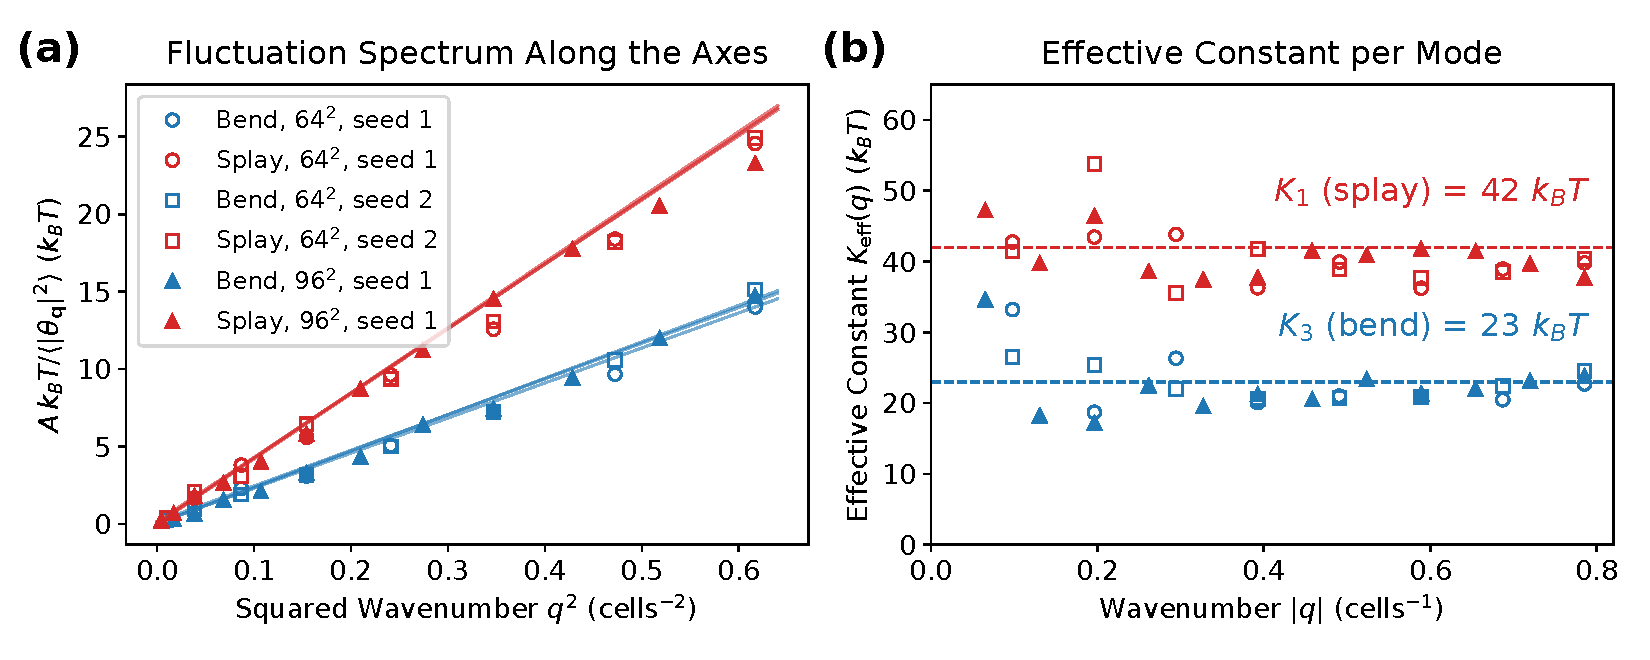
\includegraphics[width=0.85\textwidth]{../master/figs/frank_spectrum.pdf}
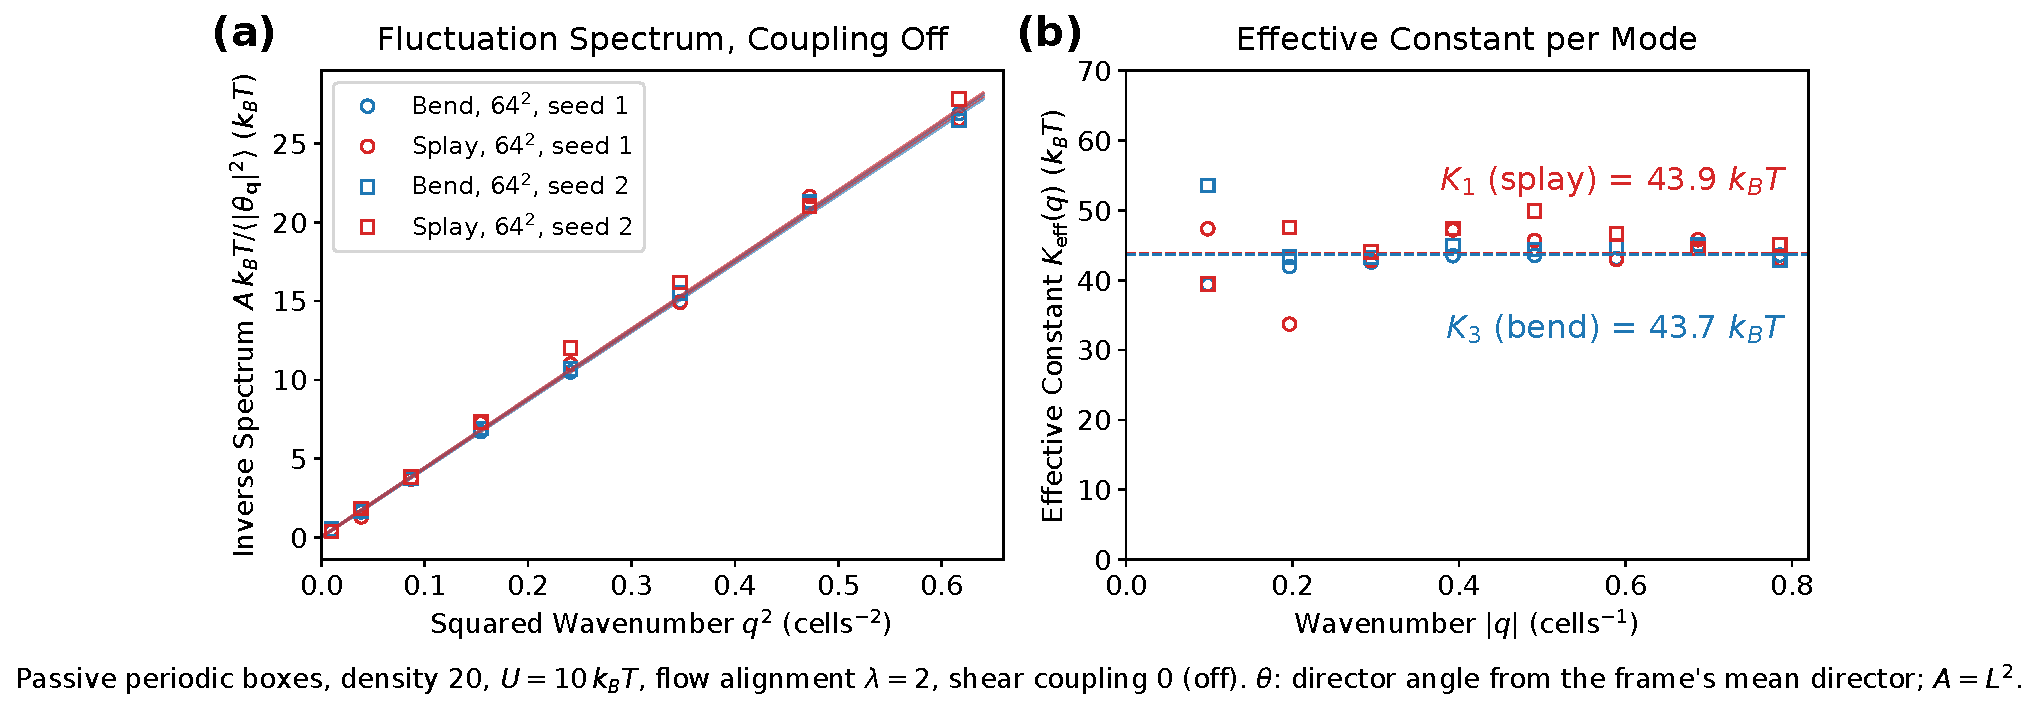
\includegraphics[width=0.85\textwidth]{../master/figs/frank_spectrum_nocoupling.pdf}
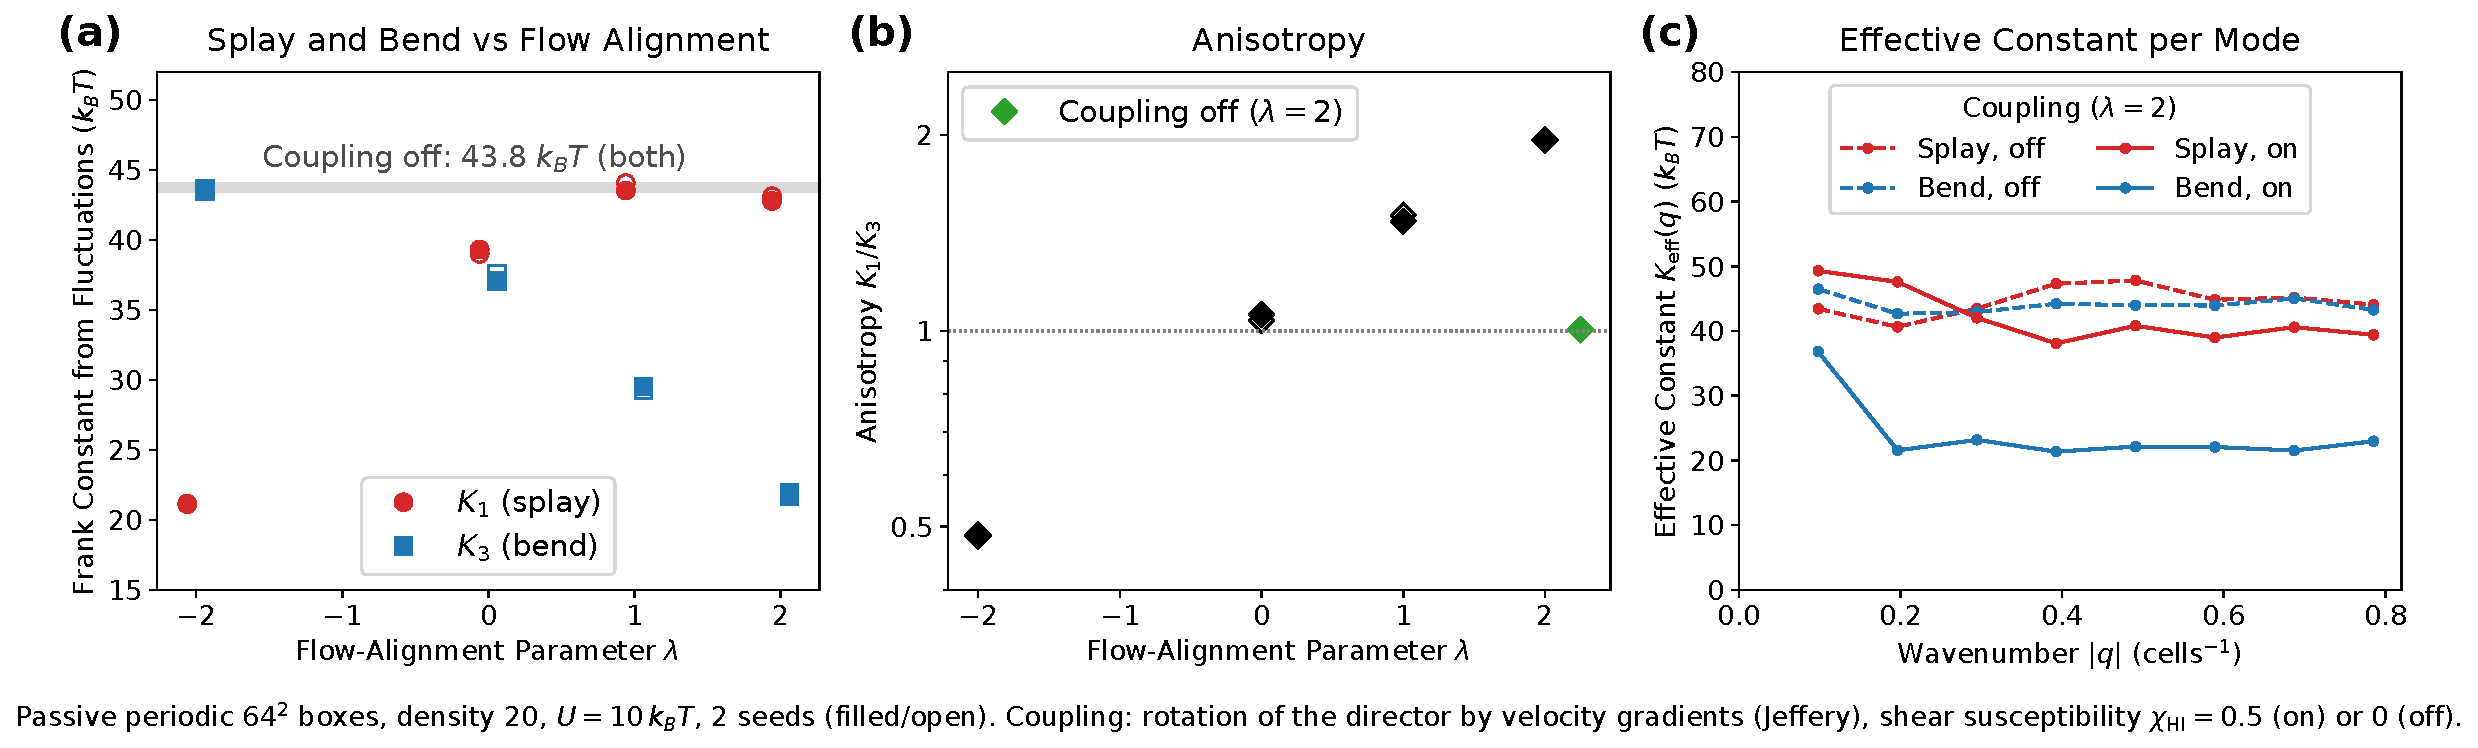
\includegraphics[width=\textwidth]{../master/figs/frank_coupling.pdf}
\caption{Top: fluctuation spectra in the director frame, coupling on (left, production) and off (right). Bottom: $K_1$, $K_3$ and $K_1/K_3$ against
$\lambda$, and $K_\mathrm{eff}(q)$ with the coupling off and on.}
\end{figure}

\clearpage\section{Claim-by-claim survey}
Columns: where the claim appears (PRL = both versions; SI; TR theory report; TiR tilt report; BR briefing; M master document section); the number now;
what it depends on; its value under reading A (bare, $K=44$, $\Delta=0$) and B (effective, $K_1=43.1$, $K_3=21.9$, $\Delta=(K_1-K_3)/2=10.6$ instead of
9.5); action. ``$\times1.35$'' is $44/32.5$ for one-constant energies. $\chi_\mathrm{HI}$ corrections apply in both readings. Rows marked \textbf{(o)} are
measurements, not affected by either reading.

{\small
\setlength{\tabcolsep}{3pt}\begin{longtable}{P{0.4cm}P{3.7cm}P{2.4cm}P{1.8cm}P{2.9cm}P{2.5cm}P{1.7cm}}
\toprule \# & Claim (where) & Now & Depends on & A: bare isotropic & B: effective & Action\\\midrule\endhead
\multicolumn{7}{l}{\textbf{1. Material constants and methods}}\\
1 & Frank constants quoted (PRL methods; SI S1; TR intro; M \S29 table) & $K_1=42$, $K_3=23$ & fluctuations, coupled & bare $K_1=K_3=44$; 42/23 are effective & 43.1/21.9 (director frame) & rewrite: both values and origin\\
2 & ``In 2D the elasticity is not isotropic'' (M \S29) & splay $\approx1.8\times$ bend & coupled measurement & false for bare MPCD & true as effective property & rewrite\\
3 & ``$K_1>K_3$ checked three ways'' (TR) & three checks & -- & none tested the bare constants (coupled fit, continuum labels, algebra) & same & rewrite\\
4 & Rotational viscosity (SI S1; TR; M \S29c) & $\gamma_1\approx60$; splay 61.9, bend 56.0 & mode decay, coupled & 58--67 off: keep 60; split came from fluctuation $K$ & keep; split partly response & keep 60, drop or explain split\\
5 & Free-defect mobility consistent with $\gamma_1$ (TR; M) & 0.0054 & $\gamma_1$ & unchanged & unchanged & none\\
6 & $\la=22.2\pm0.3$ (PRL; SI) \textbf{(o)} & measured & -- & unchanged & unchanged & none\\
7 & $\sqrt{K/\zeta_\mathrm{eff}}\approx2.8$, $\la\approx8\sqrt{K/\zeta_\mathrm{eff}}$ (M \S29) & $K=32$ & $\sqrt K$ & 3.3 cells; ratio 6.7 & unchanged & update number\\
8 & Initial director: relaxed anisotropic field (SI S1) & $K_1/K_3$ measured & -- & harmless (start only) & harmless & none\\
9 & Shendruk \& Yeomans 2015: isotropic $K$ & (not cited for this) & -- & agrees (their $w_\mathrm{HI}=0$) & agrees for bare; coupled differs & add one sentence\\
\multicolumn{7}{l}{\textbf{2. Lock and site pinning}}\\
10 & Lock $\tau_j=(2k-2)\phi_j+c$; $2|k-1|$ sites (all) & geometry & -- & unchanged & unchanged & none\\
11 & ``Site pinning needs splay $\neq$ bend'' (PRL; SI S5; TR \S2; M \S28, 29b, 29c; BR) & $\Delta=9.5$ & $K_1-K_3$ & $\Delta=0$: registry free, no static pinning; mechanism missing & $\Delta=10.6$; anisotropy induced by the flow coupling & wait for test; reword in B\\
12 & Barrier, commensurate ring (same) & 80--110 (k6), 45--70 (k8), 100--170 (k4) & $\propto\Delta$ & 0 & 90--125, 50--80, 110--190 & recompute in B; tension with rest\_pinning\\
13 & Passive $2k$ ring barrier (SI; TR; M) & $<1\,\kT$ & $\propto\Delta$ & 0 & $<1$ & conclusion holds\\
14 & Predicted collective rms vs measured (M \S29b) & 0.45--0.51 vs 0.29--0.36 & $\propto\Delta^{-1/2}$ & no prediction & 0.43--0.48 & --\\
15 & Active registry pinned, IC-independent (TR; M) \textbf{(o)} & 8 runs, $D=0.03\pm0.07$ & -- & unchanged; needs a mechanism & unchanged & --\\
16 & Passive seeded rings keep their tilt (RESEARCH 19 Oct) \textbf{(o)} & 60, $120^\circ$ held 100--300 t.u. & -- & consistent & in tension with barrier & add to discussion\\
17 & Static registry stiffness falls with crowding (SI S5; TR; BR) & 19 $\to$ 0.2--0.4\,$\kT$/rad$^2$ & $\propto\Delta$ (first order) & 0 at all $k$ & 21 $\to$ 0.2--0.45 & recompute in B\\
18 & Metropolis with $K=K_3=23$ fits tangential rms within 2--4\% (SI S5; TR; M \S29b) & no free parameter & fluctuation stiffness & still fits, but only as effective noise/stiffness of bend modes (bare 44 would give rms $\times0.72$) & unchanged & reword: evidence that the anisotropic noise acts on defects\\
19 & Wall mobility from fluctuations (SI S5; TR; M) & 0.02--0.03 & $\mu\propto1/K$ & $\approx0.010$--0.015 if bare stiffness sets relaxation; model-free 0.03 & unchanged & check\\
20 & Langevin walks, $K=K_3$, fluid noise $\times3$ (M \S29b) & normal gap & $K_3$ & recompute & unchanged & if A\\
21 & Effective-boundary stability: onset $R/\la\approx0.47$--0.50 (k6), ordering in $k$ (M \S28, 29c) & pinning $\propto\Delta/r_s^2$ & $\Delta$, $\mu$ & pinning term 0: onset and $k$-ordering need another restoring force & small shift & if A\\
22 & Particle and structured models with calibrated pinning $B=90/130$ (M \S29c) & tilt 24--29$^\circ$, onset 0.7 & $\Delta$ & recompute & unchanged & if A\\
\multicolumn{7}{l}{\textbf{3. Ejection energetics} (one constant $K=32.5$; anisotropic 42/23.1)}\\
23 & Ejection without flow (PRL; SI S6; TR; BR) & $+180$--200 (155--200) & $\propto K$ & 245--270 (210--270) & unchanged & numbers only\\
24 & Forcing a common tilt on the $2k$ ring & $+375$--475 (200--510) & $\propto K$ & 510--645 (270--690) & unchanged & numbers only\\
25 & Tilting the ejected structure & $-38$ to $+3$ & $\Delta$ & $\approx0$ (registry shift exactly free) & unchanged & --\\
26 & Ejected cheaper under a common tilt & 175--290 (20--330) & $\propto K$ & 235--395 (25--445) & unchanged & sign robust\\
27 & ``About twice the cost of ejection'' (PRL) & ratio $\approx2$ & ratio & unchanged & unchanged & none\\
28 & Mirror layer: pair $+64$--181; 12-ring $+350$--480; 14-ring cheaper 196--392 (SI S6; TR) & & $\propto K$ & 87--245; 475--650; 265--530 & unchanged & numbers only\\
\multicolumn{7}{l}{\textbf{4. Tilt angle}}\\
29 & $\tau_0=\arccos(1/\lambda)$, confirmed $\lambda=2$--6 (all) & & $\lambda$ only & unchanged & unchanged & none\\
30 & ``Elasticity alone tilts by $\approx35^\circ$'' (PRL; TR; M \S28, 29c) & $A_2\approx5\,\kT$ & $\Delta$ & $A_2\to0$ (one-constant check flat to 0.8): no static lock; ``elasticity alone does not lock the tilt'' & $A_2\approx5.6$, $\approx35^\circ$ & rewrite in A\\
31 & ``Splay $\neq$ bend adds $+2$--$3^\circ$'' (SI S7; TR; M) & 66.6/69.3 vs 64.8/66.7 & $\Delta$ & removed; one-constant flat wall gives 61--69$^\circ$ vs measured 62--64 & kept; anisotropic flat wall overshoots (69--89$^\circ$) & rewrite in A\\
32 & Boundary-layer ansatz would add $\approx16^\circ$ vs measured 2--5 (SI S7; TR; M) & $\chi\gamma_1=30$, $K=32.5$ & $\sqrt{\chi\gamma_1/K}$ & $\approx14^\circ$ & $\approx15^\circ$ ($K_\mathrm{layer}\approx38$) & conclusion unchanged\\
33 & Matching needs $\gamma_1/K=0.07$--0.18 (M \S29c) & measured 0.92 & $\chi\gamma_1/K$ & 0.68 & 0.79 & conclusion unchanged\\
34 & Leslie angle in a sheared channel \textbf{(o)} & 32.8, 29.9, $31.1^\circ$ & -- & unchanged & unchanged & none\\
\multicolumn{7}{l}{\textbf{5. Crowding drop of the tilt}}\\
35 & Drop $64.6\to44.2^\circ$; collapse on spacing; $\lambda=6$ no drop; density 40 \textbf{(o)} & measured & -- & unchanged & unchanged & none\\
36 & Fits $\tau=20+107\,d\sqrt s$ (passive), $24+59\,d\sqrt s$ (active) \textbf{(o)} & empirical & -- & unchanged & unchanged & none\\
37 & MPCD alignment length (TiR \S4; RESEARCH) & 1.4--2.7 cells & $\sqrt{K/(\chi\gamma_1)}$ & 2.3--4.4 & 2.1--4.1 & update\\
38 & MPCD core depth $d/\ell_E$ (SI S7, S8; TR; TiR) & 0.5--1.2 & $1/\ell_E$ & 0.30--0.73 & 0.33--0.79 & update\\
39 & Continuum $\zeta$ scan ``brackets'' MPCD (sparse 1.2--1.7, crowded 0.42--0.53) (SI S8; TR; TiR) & bracketing & $d/\ell_E$ & no longer: MPCD sparse $\approx$ continuum crowded, MPCD crowded below & same & rewrite\\
40 & Flat-wall continuum ($d/\ell_E\le0.29$) ``cannot reach the MPCD regime'' (SI S7; TiR) & gap & $d/\ell_E$ & gap closes (MPCD from 0.30) & from 0.33 & rewrite\\
41 & Hypothesis: sparse layers reach past $\ell_E$ ($a/2\pi=3$--8), crowded inside (1--1.6) (TiR) & $\ell_E$ 1.4--2.7 & $\ell_E$ & sparse only partly past (2.3--4.4) & 2.1--4.1 & weaker\\
42 & Continuum drop half to three-quarters of MPCD's at the same spacings (SI S8; TR; BR) & spacing-matched & -- & unchanged at matched spacing; not at matched $d/\ell_E$ & same & add caveat\\
43 & Continuum elastic models 1.82 and 0.55 (TiR; SI S8; TR; BR) & 0.55 reproduces the drop; 1.82 not & $K_1/K_3$ & MPCD's analogue is one constant: passive no drop, active one-constant disk 8--11$^\circ$ $\to$ the active one-constant disk is the matching model & unchanged (0.55 a proxy) & rewrite in A\\
44 & ``MPCD has $K_1>K_3$; a flat wall prefers $180^\circ$, so the pull comes from the circle and bulk'' (SI S8; TR; TiR; BR) & & $\Delta$ & no static Frank pull at all: the restoring torque against the flow must be dynamic & unchanged & rewrite in A\\
45 & Static tilt potential across crowding, sign change with a split bulk (TiR \S3; M \S29c): $-66/-44/-22\cos\tau$; bulk $+1$: $-46\cos\tau$ & & $\Delta$ & vanishes ($\le0.8\,\kT$) & $\times1.12$ & --\\
46 & Shear-only and $\zeta$-scan continuum controls & model units & -- & unchanged & unchanged & none\\
\multicolumn{7}{l}{\textbf{6. Elastic shielding} (one constant, $K=32.5$; SI S11; PRL Fig.~4f)}\\
47 & Circle: ideal 1.4; measured 17 (14--21); re-spaced 2.4; measured angles 16.8; jitter 7/13 & $\kT$ & $\propto K$ & 1.9; 23 (19--28); 3.2; 22.7; 9.5/17.6 & unchanged & numbers only\\
48 & Vacancy 143, extra defect 140 & & $\propto K$ & 194, 190 & unchanged & numbers only\\
49 & Ellipse: ideal 14 (27); seven even 27; measured 176 (227) & & $\propto K$ & 19 (37); 37; 238 (307) & unchanged & numbers only\\
50 & Layer force tips/flanks 7.2/6.0 (2.2/2.0) $\kT$/cell; moving a wall $+\half$ 6 cells 65 (21), 75 & & $\propto K$ & 9.7/8.1 (3.0/2.7); 88 (28), 102 & unchanged & numbers only\\
51 & Mirror: 0.3, 4.9, 27.5; measured 116, 167 (172) & & $\propto K$ & 0.4, 6.6, 37; 157, 226 (233) & unchanged & numbers only\\
52 & Shell theorem, ``the gaps, not the count, destroy shielding'' & ratios & -- & unchanged & unchanged & none\\
\multicolumn{7}{l}{\textbf{7. Escape and elastic binding} (anisotropic point-defect model 42/23.1; SI S12, S16; PRL)}\\
53 & Restoring force $F_0=-11$ to $-14\,\kT$/cell; cost drop 8--12 at departure; escape sites cheaper by 4--5 (10 at aspect 2.5) & & $K$, $\Delta$ & recompute with one constant 44 (about $\times1.35$ of the mean part) & unchanged & if A\\
54 & Depleted layer not an elastic minimum: refilling $-80$ to $-100$; ejecting 50--85; extra wall defect $-28$; Cassini 81--89; tips 73.5/75.9; flanks 7--9; vacancy neighbours $+8$--10 & & $K$, $\Delta$ & recompute; signs expected to hold & unchanged & if A\\
55 & Tips only $\approx8\%$ shallower statically & & ratio & likely unchanged & unchanged & check\\
56 & Effective wells in $\kT_\mathrm{eff}$ from escape dynamics \textbf{(o)} & 1.6--2.5 vs 0.36--0.73 & -- & unchanged & unchanged & none\\
\multicolumn{7}{l}{\textbf{8. Other}}\\
57 & Activity needed for turbulence shifted since 2024 (TODO) & unknown cause & coupling? & onset $\propto K_3/[\chi(1+\lambda)]$; a coupling change is a candidate & same & decide after test\\
58 & Leftover field $\lesssim0.06\pi K\approx6\,\kT$; approach barrier $\approx4\,\kT$ (M \S29, 30) & & $\propto K$ & 8; 5.5 (unchanged in $\pi K$) & unchanged & numbers only\\\bottomrule
\end{longtable}}

\section{What would need redoing}
\textbf{If A (bare isotropic response):}
\begin{enumerate}
\item A mechanism for the observed active site pinning (row 15) that does not use $K_1\neq K_3$; candidates: the flow-coupled effective anisotropy
acting on the defects (the Metropolis fit, row 18, suggests the noise anisotropy does act on them), core or wall-band effects, the active flow itself.
\item The restoring torque in the crowding drop (rows 44, 45) becomes purely dynamical; the active one-constant continuum disk becomes the main model
comparison (row 43).
\item Rewrite: PRL pinning sentence and Fig.~3 bands; SI S1 (constants), S5 (pinning), S6 (panel b), S7 (tilt corrections), S8 (elastic pull,
bracketing); TR \S2, \S4, summary table; TiR \S3; briefing pinning item.
\item Recompute: ejection energetics with $K=44$ (minutes; numbers only), escape/binding point-defect model (hours), stability and particle models (hours).
\end{enumerate}
\textbf{If B (effective anisotropic response):} keep the mechanism, state that the anisotropy is produced by the flow coupling (with $\lambda$ as the
control knob, which fits our $\lambda$-scan story), update $\Delta$ to 10.6, and resolve the rest\_pinning tension.

\textbf{In both:} include $\chi_\mathrm{HI}$ in $\ell_E$ (rows 37--42), quote the coupling-off constants and $\gamma_1$, cite the 2015 paper for the
isotropic bare elasticity.

\section{Status of the static response test}
Passive channel (width 40), planar or homeotropic walls, a field tilted $10^\circ$ off the wall axis; the healing length of the time-averaged profile gives
$K_1/K_3=(\xi_\mathrm{splay}/\xi_\mathrm{bend})^2$; coupling on and off, field $H=4$--16. At about 40\% of the run the fits are not yet
interpretable: the coupling-off control does not give 1 at weak field, $\xi H$ is not constant across fields, and the weakest field gives an anomalous
bulk angle. No reading is drawn from them here; the full runs and a check of the profile model come first.
\end{document}
